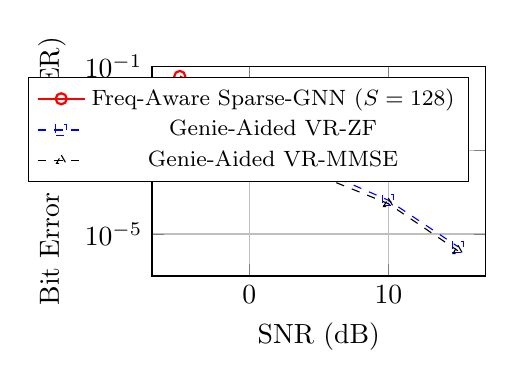
\begin{tikzpicture}
\begin{semilogyaxis}[
    xlabel={SNR (dB)},
    ylabel={Bit Error Rate (BER)},
    grid=both,
    legend style={at={(0.95,0.95)}, anchor=north east, font=\footnotesize},
    width=0.48\textwidth,
    height=0.35\textwidth,
    ymin=1e-6, ymax=1e-1
]
\addplot[color=red, mark=o, thick] coordinates {(-5, 0.057314) (0, 0.009581) (5, 0.001660) (10, 0.001225) (15, 0.001040)};
\addlegendentry{Freq-Aware Sparse-GNN ($S=128$)}
\addplot[color=blue, mark=square, dashed] coordinates {(-5, 0.029422) (0, 0.003796) (5, 0.000337) (10, 0.000064) (15, 0.000005)};
\addlegendentry{Genie-Aided VR-ZF}
\addplot[color=black, mark=triangle, dashed] coordinates {(-5, 0.028007) (0, 0.003366) (5, 0.000247) (10, 0.000053) (15, 0.000004)};
\addlegendentry{Genie-Aided VR-MMSE}
\end{semilogyaxis}
\end{tikzpicture}